


\chapter{Экспериментальная часть}\label{exp}
%\addcontentsline{toc}{chapter}{4 Экспериментальная часть}

Оценка качества работы алгоритмов.

\section{Технические характеристики}\label{texcharacters}

Технические характеристики устройства, на котором выполнялось тестирование:

\begin{enumerate}
    \item процессор: Intel® Core™ i3-7100U CPU @ 2.40GHz × 4; 
    \item память: 11,6 GiB;
    \item операционная система: Ubuntu 20.04.1 LTS.
\end{enumerate}

\section{Примеры работы}\label{examples}

На рисунке \ref{ris:w1},  \ref{ris:w2},  \ref{ris:w3},  \ref{ris:w4} и \ref{ris:w5} показан пример работы.

%\begin{figure}[H]
%    \center{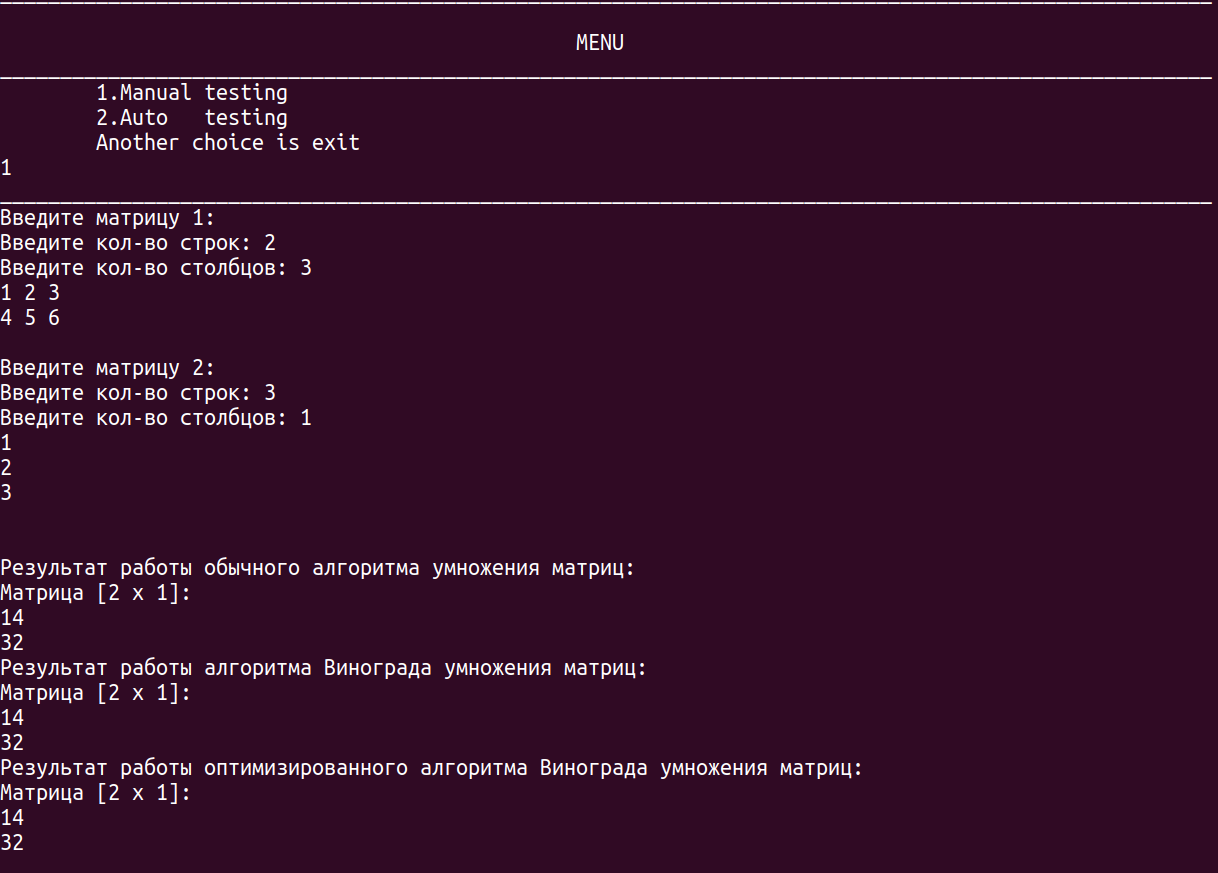
\includegraphics[scale=0.35]{w3}}
%    \caption{Ручное тестирование: тест 3}
%    \label{ris:w4}
%\end{figure}
  
\begin{figure}[H]
    \center{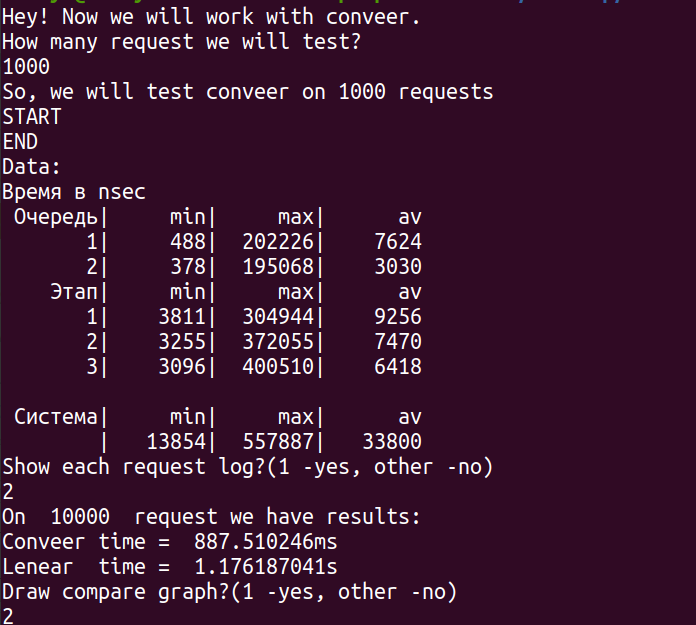
\includegraphics[scale=0.25]{w1}}
    \caption{Пример работы 1}
    \label{ris:w1}
\end{figure}
\begin{figure}[H]
    \center{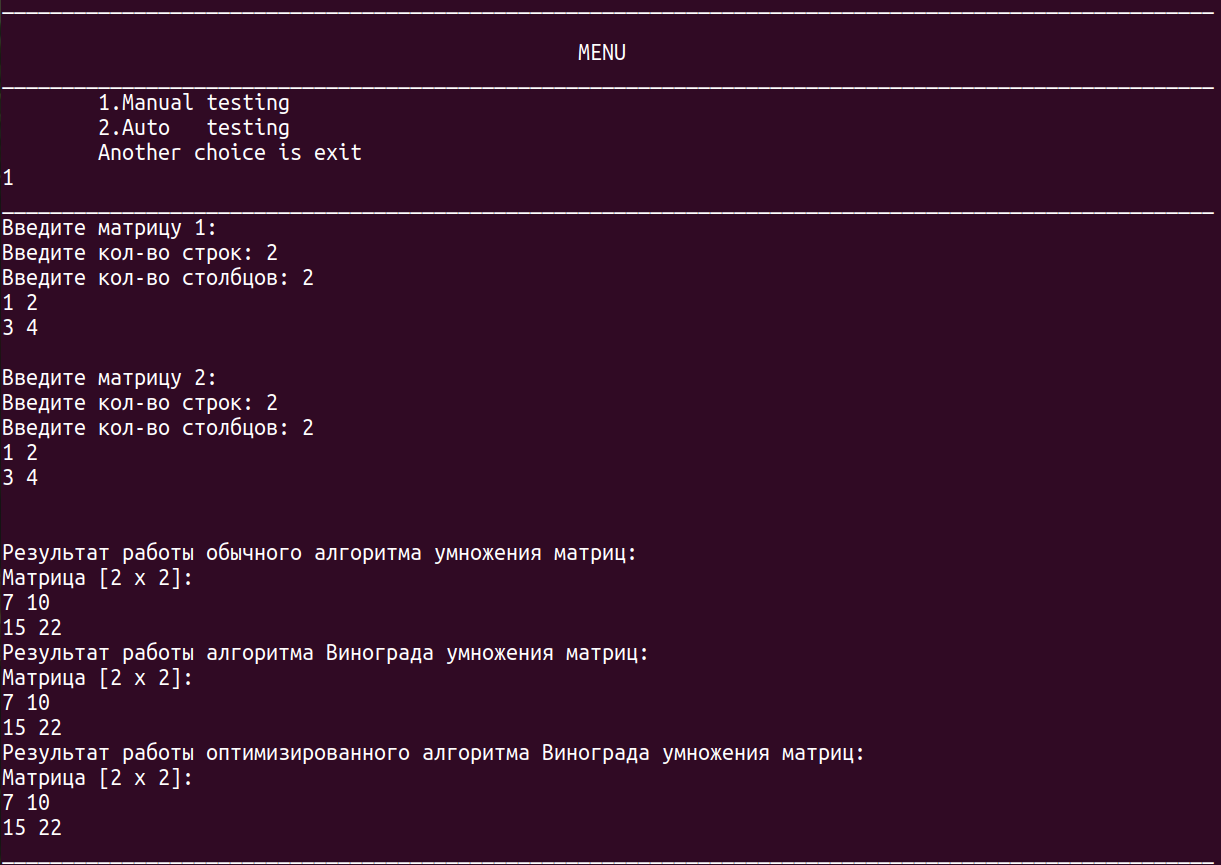
\includegraphics[scale=0.25]{w2}}
    \caption{Пример работы 2}
    \label{ris:w2}
\end{figure}

\begin{figure}[H]
    \center{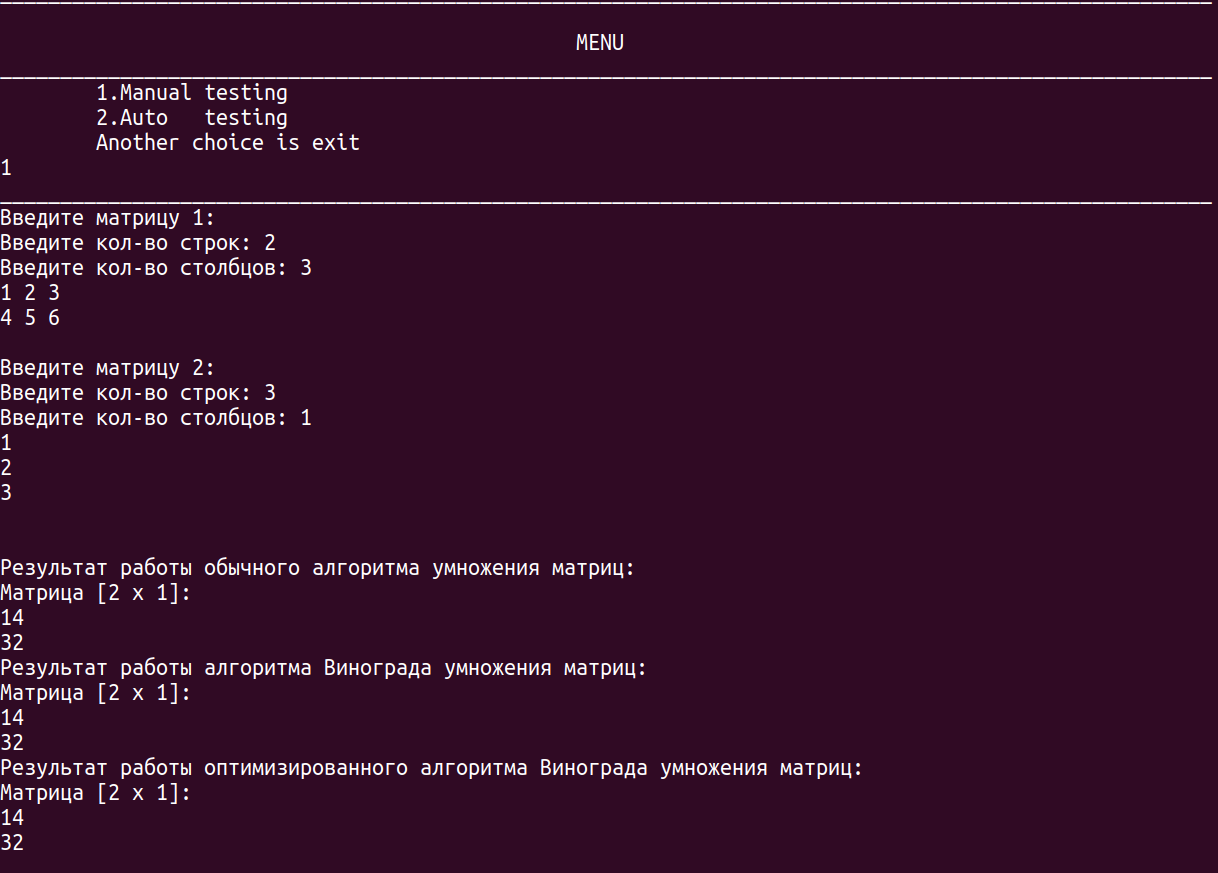
\includegraphics[scale=0.25]{w3}}
    \caption{Пример работы 3}
    \label{ris:w3}
\end{figure}

\begin{figure}[H]
    \center{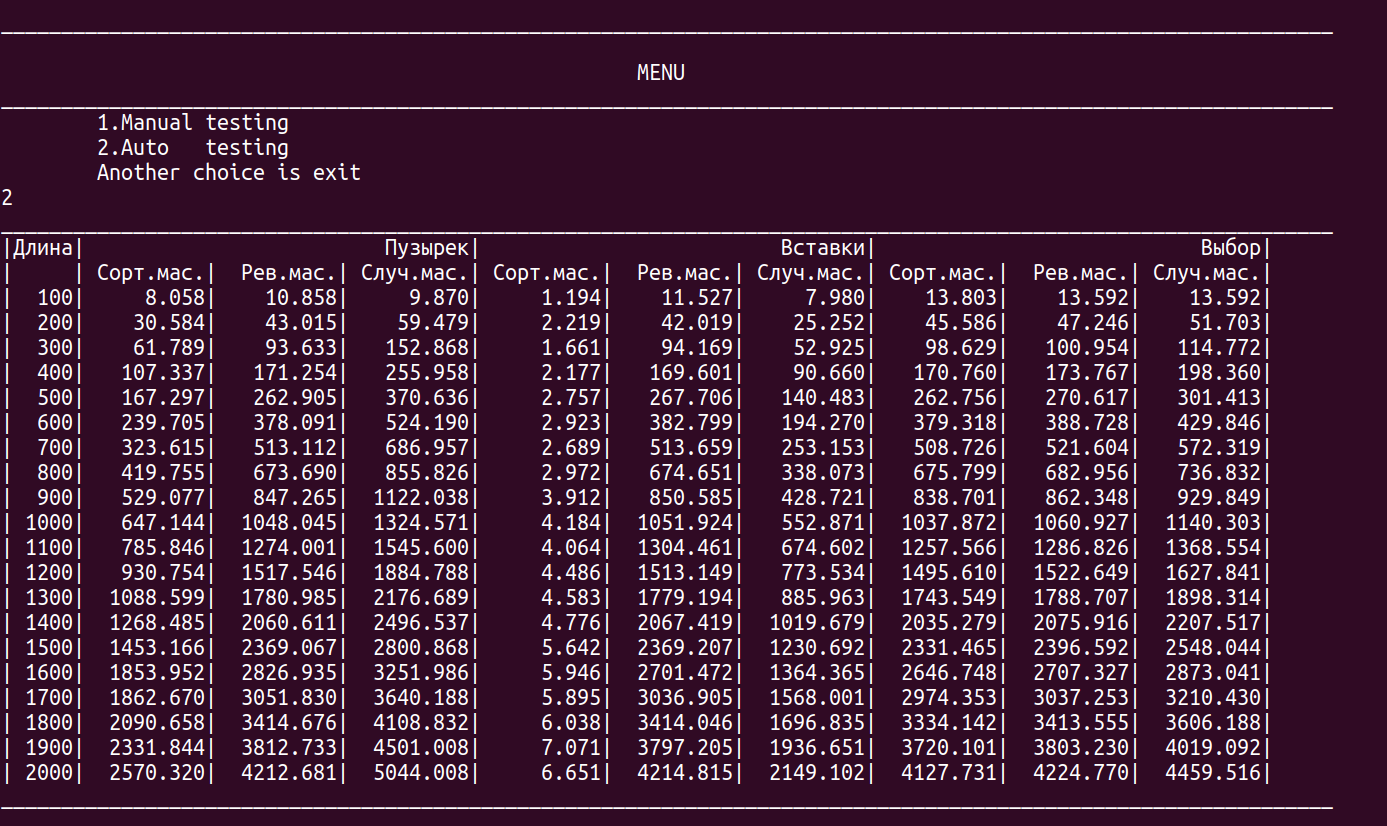
\includegraphics[scale=0.25]{w4}}
    \caption{Пример работы 4}
    \label{ris:w4}
\end{figure}

\begin{figure}[H]
    \center{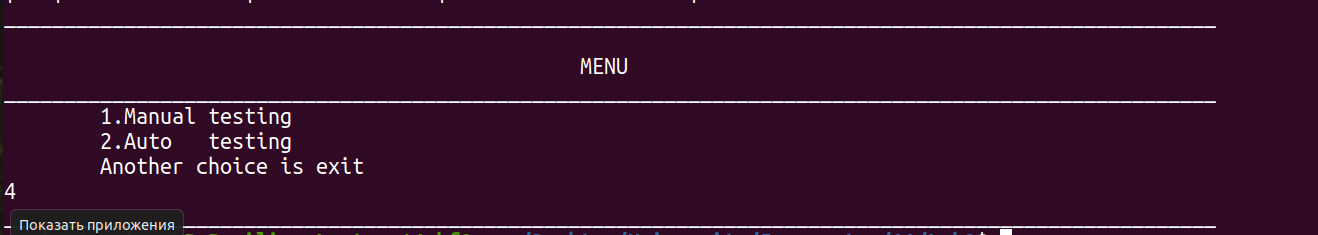
\includegraphics[scale=0.25]{w5}}
    \caption{Пример работы 5}
    \label{ris:w5}
\end{figure}

В реализованной программе 2 поток работает в 2 раза медленее остальных.
В примере 3 показана ситуация, когда диспетчер приходет слишком часто.
В примере 4 показана ситуация, когда диспетчер приходет слишком редко.
В обоих случаях, видно что 2 поток тормозит программу. В примере 5 видно, что потоки работают равномерно. 
В этом примере диспетчер работает около 1 раза на линию кирпичей.

\section{Вывод экспериментальной части}\label{experimentresult}

В данном разделе было произведен анализ реализованного алгоритма. По
результатам исследования было доказано, что алгоритм эффективно работает, если диспетчер обновляет границы участков каменщиков
один раз за укладку линии.

\addcontentsline{toc}{chapter}{{Заключение}}
\chapter*{Заключение}\label{exit}

В данной работе были изучен алгоритмы построения стены Фокса. 
Получены практические навыки реализации алгоритма с динамической балансировкой нагрузки. 
Экспериментально подтверждены различия в эффективности алгоритмов с указанием лучших и худших случаев. 
Цель работы достигнута, решены поставленные задачи. 
